\objectives{%
      \item recognize whether a learning task fits the paradigm of
            \emph{learning from examples}
            and whether it's \emph{supervised} or \emph{unsupervised}.
      \item identify within a completed learning-from-examples project:
            the \emph{training inputs(outputs)},
            \emph{testing inputs(outputs)},
            \emph{hypothesis class},
            \emph{learned hypothesis};
            and describe which parts depend on
            which.
}


\sampassage{kinds of learning}
  How do we communicate patterns of desired behavior?  We can teach:
  \begin{description}
    \item[\textbf{by instruction}:  ]  ``to tell whether a mushroom is poisonous, first look at its gills...''
    \item[\textbf{by example}:      ]  ``here are six poisonous fungi; here, six safe ones.  see a pattern?''
    \item[\textbf{by reinforcement}:]  ``eat foraged mushrooms for a month; learn from getting sick.''
  \end{description}
  %
  Machine learning is the art of programming computers to learn from such
  sources.  We'll focus on the most important case: \textbf{learning from
  examples}.\bovinenote{%
    \noparexercise{What's something you've learned by instruction?  By example?
    By reinforcement?}
    %
    In Unit 5 we'll see that learning by example unlocks the
    other modes of learning.
  }

\sampassage{from examples to predictions}
  For us, a pattern of desired behavior is a function that for each given
  situation/prompt returns a favorable action/answer.
  %
  We seek a program that, from a list of examples of prompts and matching
  answers, determines an underlying pattern.  Our program is a success if this
  pattern accurately predicts answers for new, unseen prompts.
  %
  We often define our program as a search, over some class $\hH$ of candidate
  patterns (jargon: \textbf{hypotheses}), to maximize some notion of
  ``intrinsic-plausibility plus goodness-of-fit-to-the-examples''.

  \begin{figure}[h]
    \vspace{-0.5cm}
    \par\noindent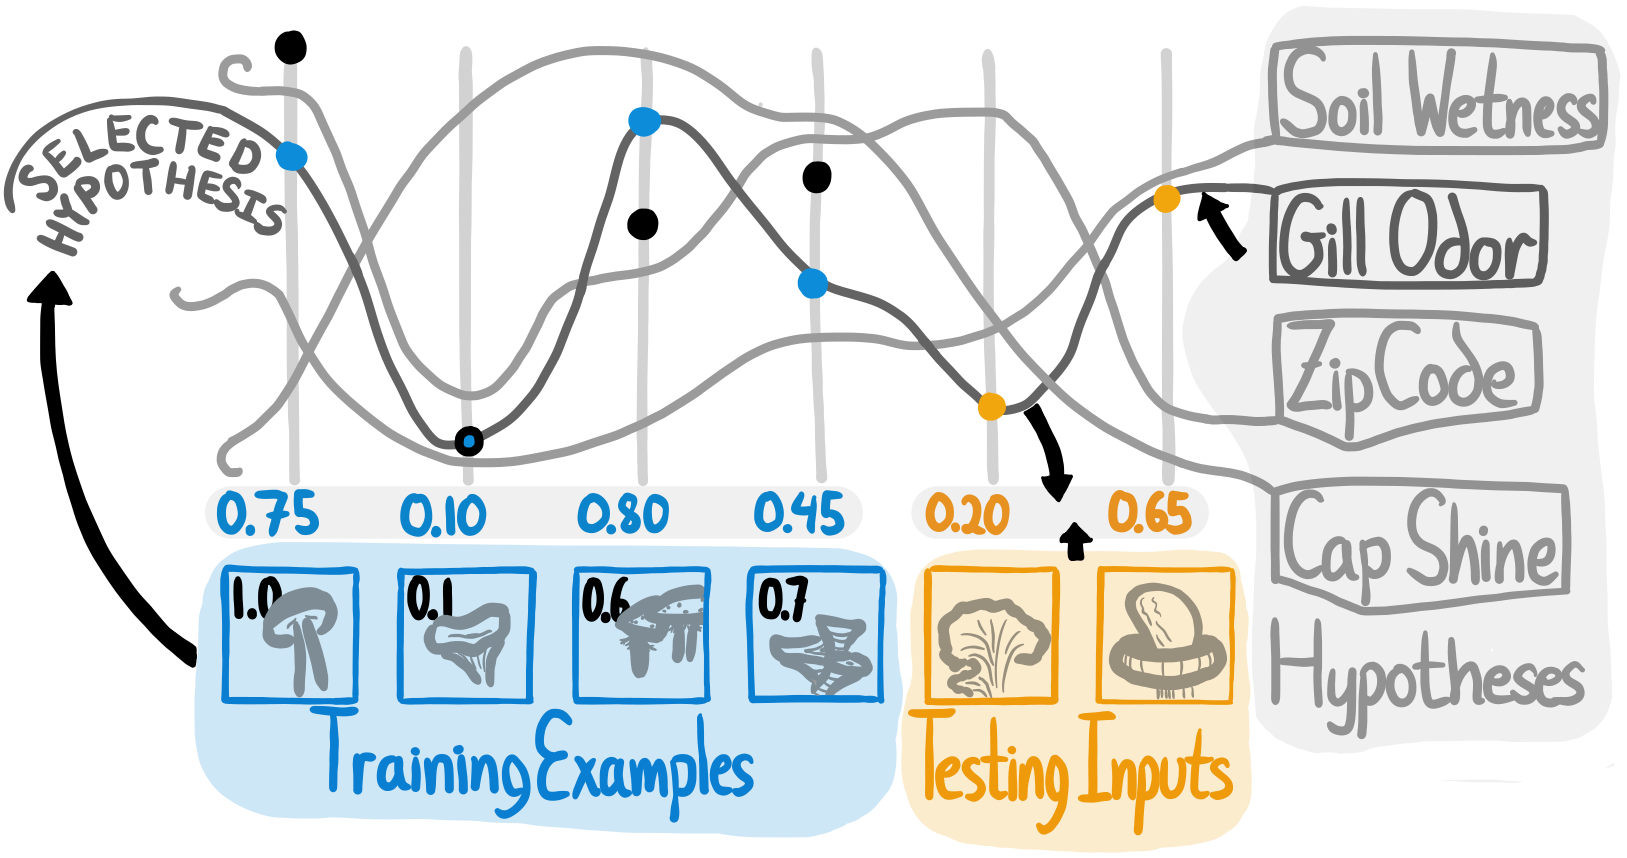
\includegraphics[width=\textwidth]{figures/ml-dataflow}
    \caption{%
      \textbf{Predicting mushrooms' poisons.}
      %
      Our learning program selects from a class of hypotheses ({\gre gray blob}) a plausible
      hypothesis that well fits (\textbf{\blu blue dots} are close to
      \textbf{black dots}) a given list of poison-labeled mushrooms ({\blu blue
      blob}).  Evaluating the selected hypothesis on new mushrooms, we predict
      the corresponding poison levels ({\rng orange numbers}).
      %
      \par The arrows show dataflow: how the hypothesis class and the
      mushroom+poisonlevel examples determine one hypothesis, which, together
      with new mushrooms, determines predicted poison levels.
      %
      Selecting a
      hypothesis is called \textbf{learning}; predicting unseen poison levels,
      \textbf{inference}.  The examples we learn from are
      \textbf{training data}; the new mushrooms and their true poison levels
      are \textbf{testing data}.
    }
    \vspace{-1.0cm}
  \end{figure}

  For example, say we want to predict poison levels (answers) of mushrooms
  (prompts).  %Comparing our `\textbf{training data}' to our
  Among our hypotheses,\bovinenote{%
      We choose four hypotheses: respectively, that
      a mushroom's poison level is
      close to:
      \par\emph{--- its ambient soil's percent water by weight};
      \par\emph{--- its gills' odor level, in kilo-Scoville units};
      \par\emph{--- its zipcode (divided by 100000)};
      \par\emph{--- the fraction of visible light its cap reflects}.
  }
  the GillOdor hypothesis fits the examples well: it guesses poison
  levels
  %(\textbf{\blu blue dots})
  close to the truth.
  %(\textbf{black dots}).
  So the program selects GillOdor.
 %(jargon: \textbf{learns})
  %The selection process is called \textbf{learning}.

  `\emph{Wait!}', you say,
  `\emph{doesn't Zipcode fit the example data more closely than GillOdor?'}.
  Yes.  But a poison-zipcode proportionality is implausible: we'd need
  more evidence before believing Zipcode.  We can easily make many oddball
  hypotheses; by chance some may fit our data well, but they probably
  won't predict well!
  %
  Thus
  ``intrinsic plausibility'' and ``goodness-of-fit-to-data''
  \emph{both}\bovinenote{%
    We choose those two notions (and our $\hH$) based on \textbf{domain
    knowledge}.  This design process is an art; we'll study some rules of
    thumb.
  } play a role in learning.

  %We must specify both notions based on our domain knowledge
  %--- this is an art but we'll learn its rules of thumb.
  %
  %We've now met ML's key elements.
  %Those are ML's elements.
  In practice we'll think of each hypothesis as mapping mushrooms to
  \emph{distributions} over poison levels; then its
  ``goodness-of-fit-to-data'' is simply the chance it allots to the
  data.\bovinenote{That's why we'll need \textbf{probability}.}
  %the details are more complex.
  We'll also use huge $\hH$s: we'll \emph{combine} mushroom features
  (wetness, odor, and shine) to make more hypotheses such as
  %Maybe
  $
    (1.0 \cdot \text{GillOdor} - 0.2\cdot \text{CapShine})
  $.\bovinenote{That's why we'll need \textbf{linear algebra}.}
  %predicts poison well!
  %
  Since we can't compute ``goodness-of-fit'' for so many hypotheses,
  we'll guess a hypothesis
  %start at a tentative hypothesis and
  then repeatedly
  nudge it up the ``goodness-of-fit'' \emph{slope}.\bovinenote{That's why we'll need \textbf{derivatives}.}
  %
  %

  %We must specify both notions based on our domain knowledge
  %--- this is an art but we'll learn its rules of thumb.
  %%
  %We'll often do this in terms of \emph{probabilities}:\bovinenote{%
  %  Still, probability isn't the only criterion: if overestimating poison
  %  levels is safer than underestimating them, then we'd want to hedge toward
  %  overestimating.
  %  This will become especially unavoidable when in Unit 5 we learn
  %  from reinforcement.
  %}
  %we supply a distribution over all hypotheses (a \textbf{prior}) and, we think
  %of each hypothesis as mapping mushrooms to \emph{distributions} over poison
  %levels.

  %\bovinenote{%
  %    \textbf{Bayesian Information Criterion}
  %}

\sampassage{supervised learning}
  We'll soon allow uncertainty by letting patterns map prompts to
  \emph{distributions} over answers.
  %\bovinenote{%
  %  Then learning programs have this type:
  %  $$
  %    \lL : (\xX\times \yY)^N \to (\xX\to \text{DistributionsOn}(\yY))
  %  $$
  %}
  %
  Even if there is only one prompt --- say, ``\emph{produce a
  beautiful melody}'' --- we may seek to learn the complicated
  distribution over answers, e.g.\ to generate a diversity of apt
  answers.  Such \textbf{unsupervised learning} concerns output
  structure.
  %
  By contrast, \textbf{supervised learning} (our main subject), concerns
  the input-output relation; it's interesting when there are many possible prompts.
  %there are many possible prompts.
  %
  Both involve learning from examples; the distinction is no more firm
  than that between sandwiches and hotdogs, but the words are good to
  know.

  %To save ink, say that $\xX$ is the set of possible prompts; $\yY$, of
  %possible answers.
  %%
  %With the example above, $\xX$ contains all
  %conceivable mushrooms and $\yY$ contains all conceivable poison
  %levels (perhaps all the non-negative real numbers).
  %%
  %If we like, we can now summarize the data flow in symbols.  A pattern is a
  %function of type $\xX\to\yY$.  And we can model the examples from which our
  %program learns as a list of type $(\xX\times \yY)^N$.  Then a program that
  %learns from examples has type:
  %$$
  %  \lL : (\xX\times \yY)^N \to (\xX\to \yY)
  %$$

%\sampassage{learning as...}
%  TODO
%    %
%\attnsam{
%    machine learning is like science.
%    %
%    machine learning is like automatic programming.
%    %
%    machine learning is like curve-fitting.
%    %%
%    three classic threads of AI
%    }
